\documentclass[a4paper,10pt]{scrartcl}
\usepackage[utf8x]{inputenc}
\usepackage[T1]{fontenc}
\usepackage{amsmath,amsfonts,amssymb,amscd,amsthm,xspace}
\usepackage[english]{babel}
\usepackage{listingsutf8}
\usepackage{color}
\usepackage{geometry}
\usepackage{graphicx}
\usepackage{multicol}
\usepackage{enumitem}
\usepackage{subfig}
\usepackage{varioref}
\usepackage{cleveref}
\usepackage{nicefrac}

%\usepackage{pst-tree}

\geometry{a4paper, left=2cm,right=2cm,top=2cm,bottom=2cm}

\newcommand{\Authors}{Robert Fels - Rollnumber: EX2014005}
\title{Principles of Embedded System Design  - Assignment 3}
\author{\Authors}
\date{\today}

\newcommand{\changefont}[3]{\fontfamily{#1} \fontseries{#2} \fontshape{#3} \selectfont}

\renewcommand{\thesection}{Task \arabic{section}}
\renewcommand{\theenumi}{(\alph{enumi})}
\renewcommand{\theenumii}{(\roman{enumii}}

\definecolor{lgray}{gray}{0.95}
\definecolor{purple}{rgb}{0.498,0,0.3333}
\definecolor{identifier}{rgb}{0,0,0.1}
\definecolor{string}{rgb}{0.192,0,1}
\definecolor{comment}{rgb}{0.25,0.5,0.37}

\pagestyle{myheadings}
\oddsidemargin\oddsidemargin
\markright{\Authors}

\lstset{
	tabsize=4, 
	frame=tlrb, 
	basicstyle=\footnotesize\changefont{pcr}{m}{n},
	breaklines=true,
	numbers=left,
	emphstyle=\textit, 
	language=Java,
	keywordstyle=\color{purple}\textbf, 
	identifierstyle=\color{identifier},
	stringstyle=\color{string},
	backgroundcolor=\color{lgray},
	showstringspaces=false,
	commentstyle=\color{comment},
	extendedchars=true,
	inputencoding=utf8/latin1
}
%\psset{nodesep=2pt,levelsep=2em,treesep=2em}

\begin{document}

\maketitle

\graphicspath{{img/}}

\section{Conflict graphs}

\paragraph{a)} 2 Colors are required as you can see below in \vref{fig:graphA}. 
\paragraph{b)} 2 Colors are required as you can see below in \vref{fig:graphB}.
\paragraph{c)} 3 Colors are required as you can see below in \vref{fig:graphC}.
	


\begin{figure}[ht!]
	\centering
	\subfloat[graph a)]{
		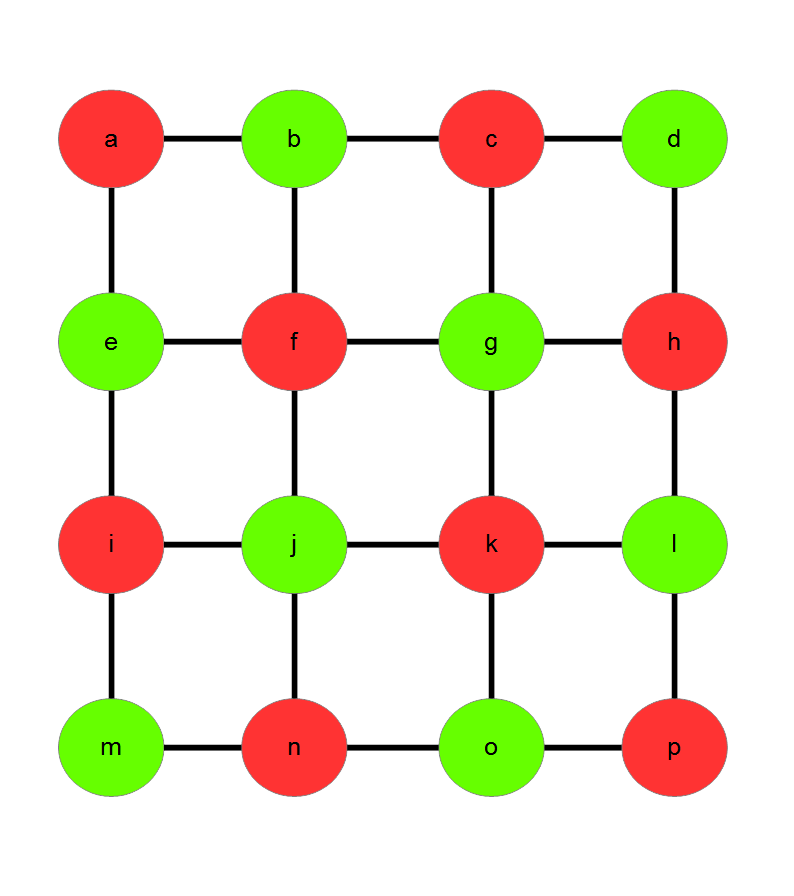
\includegraphics[scale=0.35]{graphA.png} \label{fig:graphA}
	}
	\quad
	\subfloat[graph b)]{	
		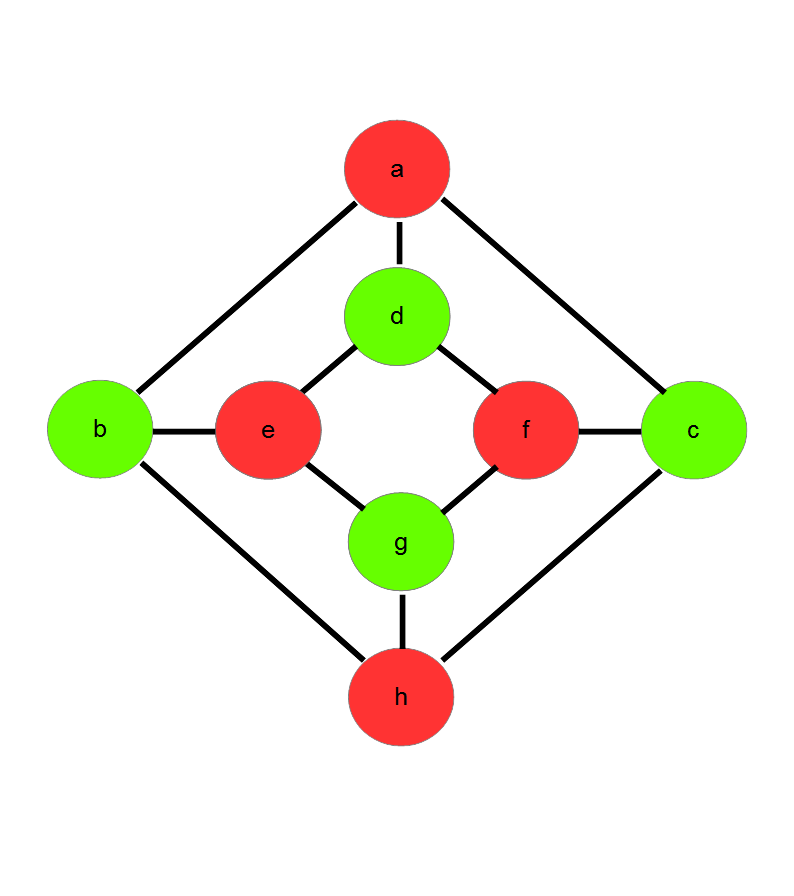
\includegraphics[scale=0.35]{graphB.png}\label{fig:graphB}
	}
	\quad
	\subfloat[graph c)]{
		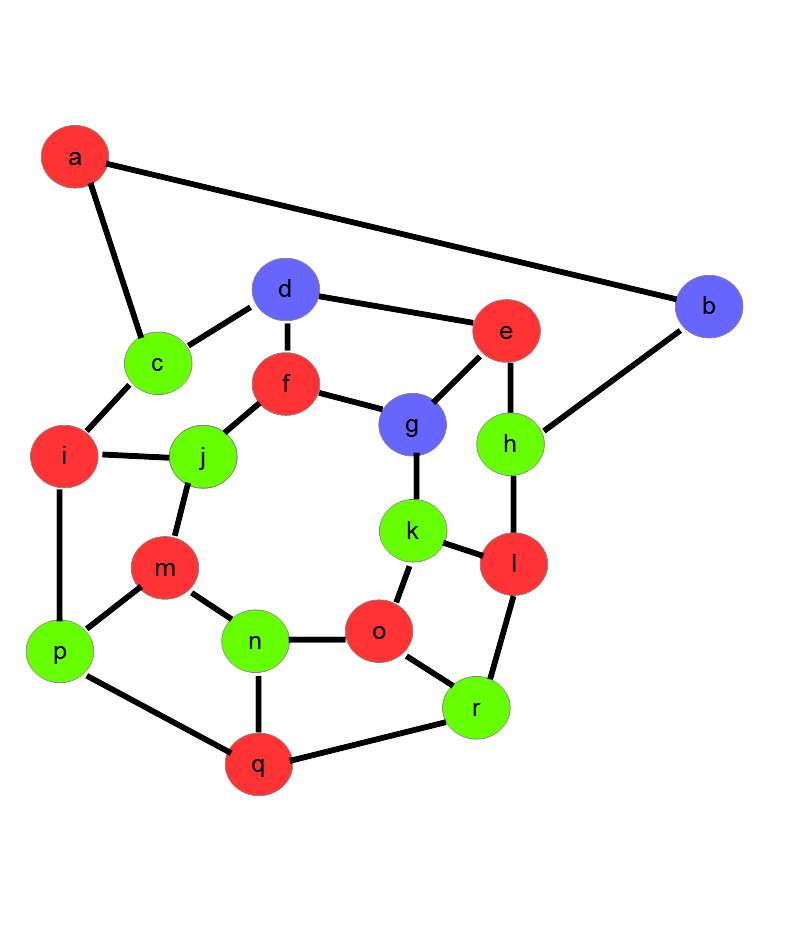
\includegraphics[scale=0.35]{graphC.png} \label{fig:graphC}
	}
	\caption{conflict graphs a), b), c)}
\end{figure}



\section{C-code examples}
	\begin{enumerate} [label=\Alph*]
		\item :
			\begin{lstlisting}
			 int a,b,c,d,e,f,g,h,i,j,k,l,m,n,o,p;
			 a=b;
			 a=e;
			 b=c;
			 b=f;
			 c=g;
			 d=c;
			 d=h;
			 e=f;
			 e=i;
			 f=g;
			 f=j;
			 g=h;
			 g=k;
			 h=l;
			 i=j;
			 i=m;
			 j=n;
			 j=k;
			 k=l;
			 k=o;
			 l=p;
			 m=n;
			 n=o;
			 o=p;
			\end{lstlisting}
		\item :
			\begin{lstlisting}
				int a,b,c,d,e,f,g,h;
				a=b;
				b=e;
				b=h;
				c=a;
				c=f;
				c=h;
				d=a;
				d=e;
				d=f;
				g=e;
				g=f;
				g=h;
			\end{lstlisting}
		\item :
			\begin{lstlisting}
				int a,b,c,d,e,f,g,h,i,j,k,l,m,n,o,p,q;
				a=b;
				a=c;
				b=h;
				c=i;
				c=d;
				d=f;
				d=e;
				e=g;
				e=h;
				f=j;
				f=g;
				g=k;
				h=l;
				i=j;
				i=p;
				j=m;
				k=l;
				k=o;
				l=r;
				m=p;
				m=n;
				n=q;
				n=o;
				o=r;
				p=q;
			\end{lstlisting}
	\end{enumerate}
\section{Reading exercise: Chapter 5 \& 6 of Wayne Wolf’s book}

\section{Scheduling with RM and EDF}
\subsection{a)}
\begin{center}
\begin{tabular}{|l|l|l|}
\hline
\textbf{Process} & \textbf{Execution time} & \textbf{Deadline} \\ 
\hline 
P1 & 1 & 3 \\ 
 
P2 & 1 & 4 \\

P3 & 2 & 6 \\
\hline
\end{tabular} 
\end{center}
$$ \dfrac{1}{3}+ \dfrac{1}{4} + \dfrac{2}{6} = \dfrac{3+4+3}{12} = \dfrac{11}{12} \approx 0,92 $$
\paragraph{RMS} 
Feasibility:
$$ 3 *(2^{\nicefrac{1}{3}}-1) = 0,78 $$

$$ 0,92 \nleq 0,78 \Rightarrow \textrm{RM-Scheduling not possible!} $$
\paragraph{EDF}  
Feasibility:
$$ \dfrac{1}{3}+ \dfrac{1}{4} + \dfrac{2}{6} = \dfrac{3+4+3}{12} = \dfrac{11}{12}$$
$$ \dfrac{11}{12} \leq 1 \: \surd $$

Scheduling:
\begin{center}
\begin{tabular}{|l|c|l|}
\hline 
\textbf{Time} & \textbf{Process} & \textbf{Deadlines} \\ 
\hline 
0 & P1 &  \\ 
1 & P2 &  \\ 
2 & P3 & P1 $\surd$ \\ 
3 & P1 & P2 $\surd$\\ 
4 & P3 &  \\ 
5 & P2 & P1 $\surd$, P3 $\surd$ \\ 
6 & P1 &  \\ 
7 & P2 & P2 $\surd$ \\ 
8 & P3 & P1 $\surd$\\ 
9 & P3 &  \\ 
10 &P1 &  \\ 
11 & idle & P1 $\surd$, P2 $\surd$, P3 $\surd$ \\ 
\hline 
\end{tabular} 
\end{center}
\subsection{b)}
\begin{center}
\begin{tabular}{|l|l|l|}
\hline
\textbf{Process} & \textbf{Execution time} & \textbf{Deadline} \\ 
\hline 
P1 & 4 & 6 \\ 
 
P2 & 2 & 8 \\

P3 & 1 & 12 \\
\hline
\end{tabular} 
\end{center}
$$ \dfrac{4}{6}+ \dfrac{2}{8} + \dfrac{1}{12} = \dfrac{12}{12} $$

\paragraph{RMS} Feasibility:
$$ 1 \nleq 0,78 \Rightarrow \textrm{RM-Scheduling not possible!} $$
\paragraph{EDF}
$$ \dfrac{4}{6}+ \dfrac{2}{8} + \dfrac{1}{12} = \dfrac{12}{12} \leq 1 \: \surd$$

Scheduling:
\begin{center}
\begin{tabular}{|l|c|l|}
\hline 
\textbf{Time} & \textbf{Process} & \textbf{Deadlines} \\ 
\hline 
0 & P1 &  \\ 
1 & P1 &  \\ 
2 & P1 & \\ 
3 & P1 & \\ 
4 & P2 &  \\ 
5 & P2 & P1 $\surd$ \\ 
6 & P1 &  \\ 
7 & P1 & P2 $\surd$ \\ 
8 & P1 & \\ 
9 & P1 &  \\ 
10 &P3 &  \\ 
11 &P2 & P1 $\surd$, P3 $\surd$ \\ 
12 &P2 &  \\ 
13 &P1 &  \\ 
14 &P1 &  \\ 
15 &P1 & P2 $\surd$\\ 
16 &P1 &  \\ 
17 &P1 & P1 $\surd$ \\ 
18 &P1 &  \\ 
19 &P1 &  \\ 
20 &P1 &  \\ 
21 &P2 &  \\ 
22 &P2 &  \\ 
23 &P3 & P1 $\surd$, P2$\surd$, P3 $\surd$ \\ 
\hline 
\end{tabular} 
\end{center}
\subsection{c)}
\begin{center}
\begin{tabular}{|l|l|l|}
\hline
\textbf{Process} & \textbf{Execution time} & \textbf{Deadline} \\ 
\hline 
P1 & 3 & 6 \\ 
 
P2 & 3 & 9 \\

P3 & 3 & 12 \\
\hline
\end{tabular} 
\end{center}
$$ \dfrac{3}{6}+ \dfrac{3}{9} + \dfrac{3}{12} = \dfrac{13}{12} $$

\paragraph{RMS}
Feasibility:
$$ \dfrac{13}{12} \nleq 0,78 \Rightarrow \textrm{RM-Scheduling not possible!} $$
\paragraph{EDF}
Feasibility:
$$ \dfrac{13}{12} \nleq 1 \Rightarrow \textrm{EDF-Scheduling not possible!} $$
\section{C-code for RM and EDF}
Please see the attachments of the Mail and find the code there.


\end{document}